\documentclass[11pt, oneside]{article}   	% use "amsart" instead of "article" for AMSLaTeX format
\usepackage{geometry}                		% See geometry.pdf to learn the layout options. There are lots.
\geometry{letterpaper}                   		% ... or a4paper or a5paper or ... 
%\geometry{landscape}                		% Activate for for rotated page geometry
%\usepackage[parfill]{parskip}    		% Activate to begin paragraphs with an empty line rather than an indent
\usepackage{graphicx}				% Use pdf, png, jpg, or eps� with pdflatex; use eps in DVI mode
								% TeX will automatically convert eps --> pdf in pdflatex		
\usepackage{amssymb}
\usepackage{amsmath}

\title{Hyperbola}
%\author{The Author}
\date{}							% Activate to display a given date or no date

\graphicspath{{/Users/telliott_admin/Dropbox/Tex/png/}}

\begin{document}

\maketitle
%\section{}
% \subsection*{R code}
% \begin{lstlisting}  \end{lstlisting}
% \begin{center} 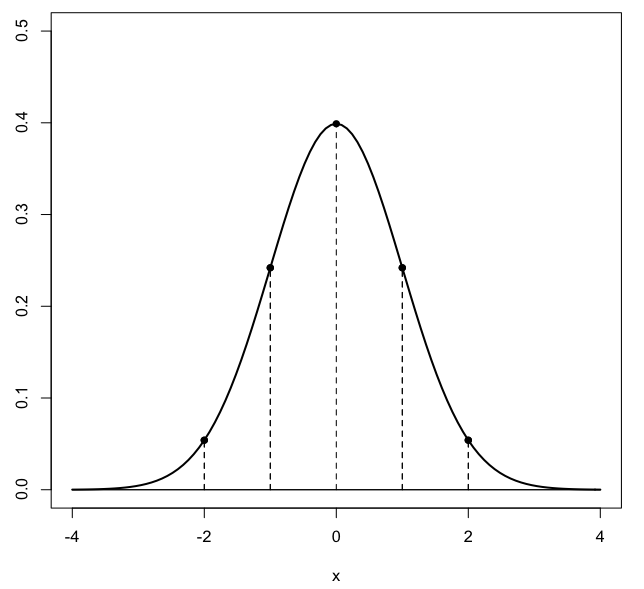
\includegraphics [scale=0.4] {gauss3.png} \end{center}
% \begin{bmatrix} a  &  b \\ c  &  d \end{bmatrix}
% \bigg |_

\large
\noindent
Here is a hyperbola as shown in the wikipedia article on the subject.
\begin{center} 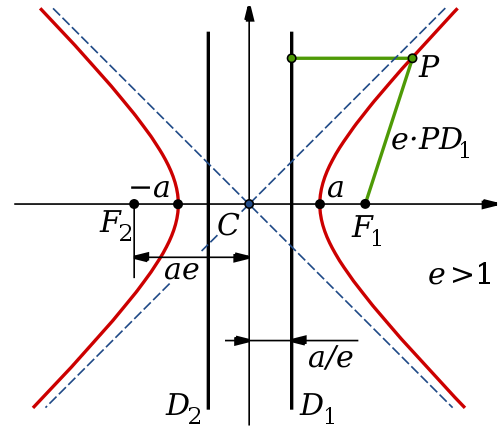
\includegraphics [scale=0.4] {hyper.png} \end{center}
Hyperbolas of this type (that open "east-west") have equations of the form
\[ \frac{x^2}{a^2} - \frac{y^2}{b^2} = 1 \]
We can see that 
\[ \frac{x^2}{a^2} = 1 + \frac{y^2}{b^2}\]
so that the minimum value of $x$ occurs when $y=0$ and $x=a$.  The conjugate hyperbola of this one is
\[ \frac{x^2}{a^2} - \frac{y^2}{b^2} = -1 \]
or equivalently 
\[ -\frac{x^2}{a^2} + \frac{y^2}{b^2} = 1 \]
opens "north-south."  And, although I want to wait to deal with this complication, we have to mention another very common hyperbola
\[ xy = c \]
where it must be true that $x \ne 0$ and $y \ne 0$.

Another feature of hyperbolas is the asymptote, the straight line which is approached when $x,y >> a,b$.  In the case of the first example
\[ \frac{y^2}{b^2} = \frac{x^2}{a^2} - 1 \]
\[ y^2 = \frac{b^2}{a^2} x^2 - \frac{1}{a^2} \]
but for large $x$ and $y$ this approaches
\[ y^2 = \frac{b^2}{a^2} x^2 \]
\[ y = \pm \frac{b}{a} x \]


\end{document}  